\documentclass{article}
\usepackage{amsmath}
\usepackage{amssymb}
\usepackage{bm}
\usepackage{amsthm}
\usepackage{enumerate}
\usepackage{graphicx}
\usepackage{psfrag}
\usepackage{color}
\usepackage{url}
\usepackage{listings}
\usepackage{xcolor}
\usepackage{tikz}
\usetikzlibrary{positioning}
\usetikzlibrary{tikzmark}
\tikzset{main node/.style={circle,fill=gray!20,draw,minimum size=.75cm,inner sep=0pt},}

\definecolor{codegreen}{rgb}{0,0.5,0}
\definecolor{codewhite}{rgb}{1,1,1}
\definecolor{codegray}{rgb}{0.5,0.5,0.5}
\definecolor{codepurple}{rgb}{0.58,0,0.82}
\definecolor{codeblack}{rgb}{0,0,0}
\definecolor{codeorange}{rgb}{0.8,0.4,0}

\lstdefinestyle{mystyle}{
    backgroundcolor=\color{codewhite},   
    commentstyle=\color{codegray},
    keywordstyle=\color{codegreen},
    numberstyle=\color{codegray},
    stringstyle=\color{codeorange},
    basicstyle=\ttfamily ,
    breakatwhitespace=false,         
    breaklines=true,                 
    captionpos=b,                    
    keepspaces=true,                 
    numbers=left,                    
    numbersep=5pt,                  
    showspaces=false,                
    showstringspaces=false,
    showtabs=false,                  
    tabsize=4
}
\lstset{style=mystyle}


\setlength{\hoffset}{-1in}
\addtolength{\textwidth}{1.5in}
\setlength{\voffset}{-1in}
\addtolength{\textheight}{1.5in}
\newcommand{\be}{\begin{enumerate}}
\newcommand{\ee}{\end{enumerate}}
\newcommand{\BigO}[1]{\ensuremath\mathcal{O}\left(#1\right)}
\newcommand{\il}[1]{\lstinline!#1!}
\newcommand{\gnorm}[1]{\left|\left|#1\right|\right|}
\newcommand{\abs}[1]{\left|#1\right|}
\newcommand{\parens}[1]{\left(#1\right)}
\newcommand{\bracks}[1]{\left\{#1\right\}}
\newcommand{\sqbracks}[1]{\left[#1\right]}
\newcommand{\vep}{\varepsilon}
\newcommand{\ceiling}[1]{\left\lceil#1\right\rceil}
\newcommand{\R}{\mathbb{R}}
\newcommand{\N}{\mathbb{N}}
\newcommand{\Z}{\mathbb{Z}}
\newcommand{\distrib}[2]{\text{#1}\left(#2\right)}
\newcommand{\dd}[1]{\frac{d}{d#1}}
\newcommand{\abracks}[1]{\left< #1\right>}

\begin{document}
	\begin{center}
		\textbf{Spring 2020, CS 310:\ Homework 5 \& 6} \\
		\textbf{Due:\ Thursday, May 7th, 2020} \\
		\textbf{Joseph Diaz: 819947915}
	\end{center}
\noindent\makebox[\linewidth]{\rule{\paperwidth}{0.4pt}}
\be[1.]
	\item Represent the Following graph as both adjacency matrix and adjacency list. Make sure to label which is the list and which is the matrix.
	\begin{figure}[h]
	\centering
	\includegraphics[width=.9\linewidth]{"PlaneGraph".jpg}
	\end{figure}
	\begin{proof}[Solution]
	Here we have the adjacency matrix for the graph above:
	$$\begin{tabular}{c|cccccc}
	  & A & B & C & D & E & F\\ \hline
	A & 0 & 1 & 2 & 0 & 0 & 3 \\
	B & 1 & 0 & 0 & 2 & 0 & 0 \\
	C & 2 & 0 & 0 & 6 & 3 & 0 \\
	D & 0 & 2 & 6 & 0 & 4 & 0 \\
	E & 0 & 0 & 3 & 4 & 0 & 5 \\
	F & 3 & 0 & 0 & 0 & 5 & 0 
	\end{tabular}$$
	Now let $\parens{e, V}$ be the elements of each vertex's edge list, where $e$ is the weight of the edge and $V$ is the vertex connected; so the adjacency list is:
	\begin{center}
	\begin{tabular}{c|cccccccc}
	\underline{Start} &\\
	$\downarrow$ & \\
	A & $\to$ & (1,B) & $\to$ & (2,C) & $\to$ & (3, F) & $\to$ & \il{null} \\
	$\downarrow$ & \\
	B & $\to$ & (1,A) & $\to$ & (2,D) & $\to$ & \il{null} \\
	$\downarrow$ & \\
	C & $\to$ & (2,A) & $\to$ & (6,D) & $\to$ & (3,E) & $\to$ & \il{null} \\
	$\downarrow$ & \\
	D & $\to$ & (2,B) & $\to$ & (6,C) & $\to$ & (4,E) & $\to$ & \il{null} \\
	$\downarrow$ & \\
	E & $\to$ & (3,C) & $\to$ & (4,D) & $\to$ & (5,F) & $\to$ & \il{null}\\
	$\downarrow$ & \\
	F & $\to$ & (3,A) & $\to$ & (5,E) & $\to$ & \il{null}\\	
	\end{tabular}

	\end{center}
	\end{proof}
		
	\item Which of the following is true about the graph in Question 1?
	\be[a.]
		\item It is a weighted directed graph
		\item It is an unweighted undirected graph
		\item \tikzmarknode[fill=cyan,fill
opacity=0,draw=black!60!black,thick,rounded corners,inner sep=2pt,text
opacity=1]{test}{It is a weighted undirected graph}
		\item It is an unweighted directed graph
	\ee
	
	\item Use the following graph to answer all questions in this part.
	\begin{figure}[h]
	\centering
	\includegraphics[width=.9\linewidth]{"PlaneGraph3".jpg}
	\end{figure}
	\be[a.]
		\item Use the Prim’s Algorithm to find the Minimum Spanning Tree of the above graph.
Show the order in which the nodes are discovered and then draw the final result of the algorithm along with the weights.
	\begin{proof}[Solution]
	Here we start with A, and the order in which the other vertices are discovered and added are:
	\begin{center}
	[A, C, B, E, D, F]
	\end{center}
	And the tree we get is:
	\begin{center}
	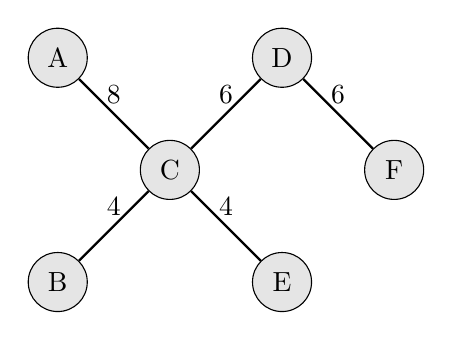
\begin{tikzpicture}
	
	\begin{scope}[xshift=0]
    \node[main node] (1) {C};
    \node[main node] (2) [above left = 1.25cm  of 1] {A};
    \node[main node] (3) [below right = 1.25cm  of 1] {E};
    \node[main node] (4) [below left = 1.25cm  of 1] {B};
    \node[main node] (5) [above right = 1.25cm  of 1] {D};
    \node[main node] (6) [below right = 1.25cm  of 5] {F};


    \path[draw,thick]
    (1) edge node[above] {8} (2)
    (1) edge node[above] {4} (3)
    (1) edge node[above] {4} (4)
    (1) edge node[above] {6} (5)
    (6) edge node[above] {6} (5)
    ;
    \end{scope}
	\end{tikzpicture}
	\end{center}

	\end{proof}

		\item Use the Kruskal’s Algorithm to find the Minimum Spanning Tree of the above graph.
Show the order in which the nodes are discovered and then draw the final result of the algorithm along with the weights.
		\begin{proof}[Solution]
		The first edge added is (B,C), and the order in which the other vertices are discovered and added are:
	\begin{center}
	[B, C, E, D, F, A]
	\end{center}
	And the tree we get is:
	\begin{center}
	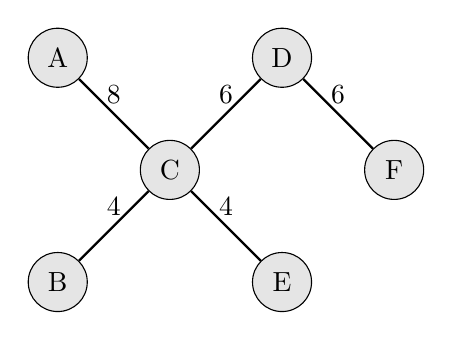
\begin{tikzpicture}
	
	\begin{scope}[xshift=0]
    \node[main node] (1) {C};
    \node[main node] (2) [above left = 1.25cm  of 1] {A};
    \node[main node] (3) [below right = 1.25cm  of 1] {E};
    \node[main node] (4) [below left = 1.25cm  of 1] {B};
    \node[main node] (5) [above right = 1.25cm  of 1] {D};
    \node[main node] (6) [below right = 1.25cm  of 5] {F};


    \path[draw,thick]
    (1) edge node[above] {8} (2)
    (1) edge node[above] {4} (3)
    (1) edge node[above] {4} (4)
    (1) edge node[above] {6} (5)
    (6) edge node[above] {6} (5)
    ;
    \end{scope}
    
	\end{tikzpicture}
	\end{center}
	
	\end{proof}
		\item Are your answers in 3 (a) and 3(b) the same?
		\begin{center}
		Yes, they are exactly the same.
		\end{center}
		
		\item If you answered yes to 3(c), explain why and when they will be different. If you answered no to 3(c), explain why and when they will be the same?
		\begin{proof}[Solution]
		For a given undirected graph with weighted edges, the algorithms can give different tree only if (not if and only if) the graph has indistinct edge weights. In other words, any case in which 2 edges have the same weight allows for the possibility that one edge will be added to the MST with one algorithm and not added in with the other algorithm. So there is the potential that you'll have 2 different spanning trees from the same graph; they will, however, have the same cost. The graph that we use the algorithms on in this question has the potential to produce different MST's with the different algorithms, but it's purely through serendipity that they turned out the same.
		\end{proof}
	\ee
	
	\item Hashing \\
The properties of the hashtable for this question are as follows:
	\be[(i)]
		\item \il{Size = 12}
		\item \il{Collison Resolution Method: Open Addressing}
		\item \il{Hash functions: H(k) = |3 - (k mod 12)|}
	\ee
	The following keys have to be inserted into the Hash Table \textbf{in sequence}:
	$$33,\ 10,\ 9,\ 13,\ 12,\ 45,\ 26,\ 17$$

	Fill the values in the Hash Table below, also \textbf{showcase the working} of how you find the index for each value inserted.
	\begin{center}
	\begin{tabular}{c|c}
	
	
		\begin{tabular}{|c|c|}
		\hline
		index & key \\
		\hline
		0 & \\
		\hline
		1 & 26\\
		\hline
		2 & 13\\
		\hline
		3 & 12\\
		\hline
		4 & 17\\
		\hline
		5 & \\
		\hline
		6 & 33\\
		\hline
		7 & 10\\
		\hline
		8 & 9\\
		\hline
		9 & 45\\
		\hline
		10 & \\
		\hline
		11 & \\
		\hline
		\end{tabular}
		&
		\begin{tabular}{c|l}
		$k$ & Hash Function and linear probing\\
		\hline
		33 & $\to\ H(33) = \abs{3 - (33 \mod 12)} = 6$, index 6 is free, insert $33$ at index 6.\\
		
		10 & $\to\ H(10) = \abs{3 - (10 \mod 12)} = 7$, index 7 is free, insert $10$ at index 7.\\
		
		9 & $\to\ H(9) = \abs{3 - (9 \mod 12)} = 6$, index 6 is taken.\\
		
		 & $\to$ check index 7, index 7 is taken.\\
		
		 & $\to$ check index 8, index 8 is free, insert $9$ at index 8.\\
		
		13 & $\to\ H(13) = \abs{3 - (13 \mod 12)} = 2$, index 2 is free, insert $13$ at index 2.\\
		
		12 & $\to\ H(12) = \abs{3 - (12 \mod 12)} = 3$, index 3 is free, insert $12$ at index 3.\\
		
		45 & $\to\ H(45) = \abs{3 - (45 \mod 12)} = 6$, index 6 is taken.\\ 
		& $\to$ check index 7, index 7 is taken.\\
		& $\to$ check index 8, index 8 is taken.\\
		& $\to$ check index 9, index 9 is free, insert $45$ at index 9.\\
		
		26 & $\to\ H(26) = \abs{3 - (26 \mod 12)} = 1$, index 1 is free, insert $26$ at index 1.\\
		
		17 & $\to\ H(17) = \abs{3 - (17 \mod 12)} = 2$, index 2 is taken.\\
		
		 & $\to$ check index 3, index 3 is taken.\\
		
		 & $\to$ check index 4, index 4 is free, insert $17$ at index 4.\\
		\end{tabular}
	\end{tabular}
	\end{center}
	Do you think the above Hash Function is effective? What could make it better? What in your opinion is a “good” hash function?
	\begin{proof}[Solution]
	The hash function above is not effective. For starters, the definition of $H(k)$ constrains the number of possible hash codes to $0, \cdots,\ 8$. Let $f(k) = 3 - (k \mod 12),\ k \in \Z$ then, the largest value that $\parens{k \mod 12}$ could be is 11, and the smallest it could be is 0, which implies: 
	$$ -8 \leq f(k) \leq 3$$
	Clearly, $H(k) = \abs{f(k)}$, so:
	$$0 \leq H(k) \leq 8$$
	So, by itself, $H(k)$ would never be able to map to indices 9, 10, or 11. The only way we were able to insert an element at 9 above was through linear probing for an empty spot, because 6, 7, and 8 were already taken. The lack of coverage is made worse when you consider that using the absolute value can cause more collisions as the positive and negative version of the same number will both resolve to the same hash code. This  could be made better by redefining $H(k)$ like so:
	$$H(k) = f(k) \mod 12$$
	This way $H(k)$ can map a key to every hash code index in the hash table, and given random keys, each hash code is theoretically equally likely. That being said, collisions are still likely because our hash table only has space for 12 elements and the keys we're dealing with are all integers. \\\\
	A good hash function is one whose outputs are equally likely given random keys, as that allows for the elements added to the hash table to be as evenly spread out as possible. This reduces the potential for collisions, and improves the performance of basically every other operation on hash tables (insertion, deletion, searching, etc). Using the data that's actually being hashed in the hash function is also crucial. For each key you could hypothetically generate a random hash value with out using the data itself, but that would mean that 2 different keys could potentially have the same hash code and that's counter-productive. Similar keys should also generate hash codes that are as different as possible, this again helps spread the elements of the hash table around and in the case of hashing passwords that means greater security as it's more difficult to determine the hash function being used.
	\end{proof}
	
	\item Dijkstra’s Algorithm
	\begin{figure}[h]
	\centering
	\includegraphics[width=.9\linewidth]{"dijk new".jpg}
	\end{figure}
	
	Calculate the single shortest path from A to every other vertex in the above graph using Dijkstra’s algorithm.
Show the steps in the table given below, cross out old values and fill new ones as better paths are discovered through the algorithm.
Once you have stepped through the whole algorithm, write the lowest cost path from A to F.\\\\
	Order in which the vertices are discovered: [A, B, C, G, E, F, D]
	\begin{center}
	Here we use the $\to$ symbol to represent a change from the value on the left to the value on the right.\\
	\begin{tabular}{|c|c|l|l|}
	\hline
	Vertex & Known  & Cost & Path \\
	\hline
	A & T $\to\ Y_1$ & $\infty \to 0$ & nil \\
	\hline
	B & T $\to\ Y_2$ & $\infty \to 1$ & nil $\to$ A\\
	\hline
	C & T $\to\ Y_3$ & $\infty \to 3 \to 2$ & nil $\to$ A $\to$ B\\
	\hline
	D & T $\to\ Y_7$ & $\infty \to 8$ & nil $\to$ B\\
	\hline
	E & T $\to\ Y_5$ & $\infty \to 6 \to 5$ & nil $\to$ B $\to$ C\\
	\hline
	F & T $\to\ Y_6$ & $\infty \to 10 \to 7$ & nil $\to$ A $\to$ E\\
	\hline
	G & T $\to\ Y_4$ & $\infty \to 3$ & nil $\to$ B\\
	\hline
	\end{tabular}
	\end{center}
	Shortest Path from A to F is: \underline{A $\to$ B $\to$ C $\to$ E $\to$ F, Cost: 7}
\ee
\noindent\makebox[\linewidth]{\rule{\paperwidth}{0.4pt}}
	
\end{document}
